\usetikzlibrary{calc}

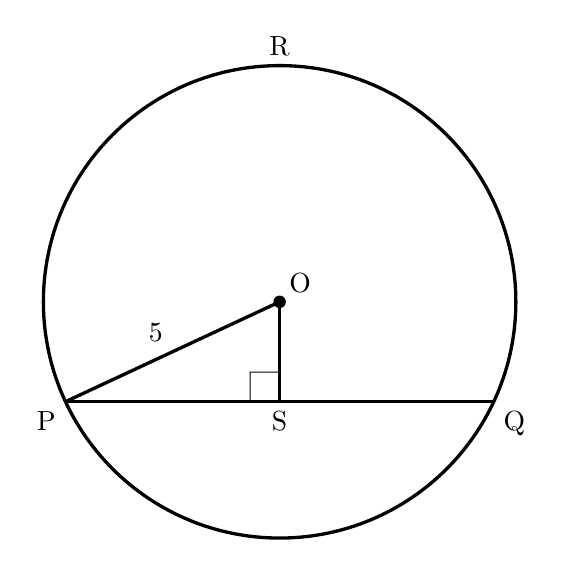
\begin{tikzpicture}[scale=1.5]

% Define radius
\pgfmathsetmacro{\radius}{2}

% Center of circle
\coordinate (O) at (0,0);

% Points on circle using polar coordinates (angle:radius)
\coordinate (P) at (205:\radius);
\coordinate (Q) at (335:\radius);
\coordinate (R) at (90:\radius);

% S is projection of O onto line PQ
\coordinate (S) at ($(P)!(O)!(Q)$);

% Draw circle
\draw[very thick] (O) circle (\radius);

% Draw line PQ (extended beyond circle)
\draw[very thick] (P) -- (Q);

% Draw line segment OP
\draw[very thick] (O) -- (P);

% Draw perpendicular line OS
\draw[very thick] (O) -- (S);

% Right angle symbol at S
\coordinate (S1) at ($(S)!2.5mm!(P)$);
\coordinate (S2) at ($(S)!2.5mm!(O)$);
\coordinate (S3) at ($(S1)+(S2)-(S)$);
\draw (S1) -- (S3) -- (S2);

% Filled point at O
\fill (O) circle (1.5pt);

% Labels
\node[above right] at (O) {O};
\node[above] at (R) {R};
\node[below left] at (P) {P};
\node[below right] at (Q) {Q};
\node[below] at (S) {S};
\node[above left] at ($(O)!0.5!(P)$) {5};

\end{tikzpicture}